\documentclass[../main.tex]{subfiles}
\begin{document}
\section{Meccanica}
\begin{figure}
    \centering
    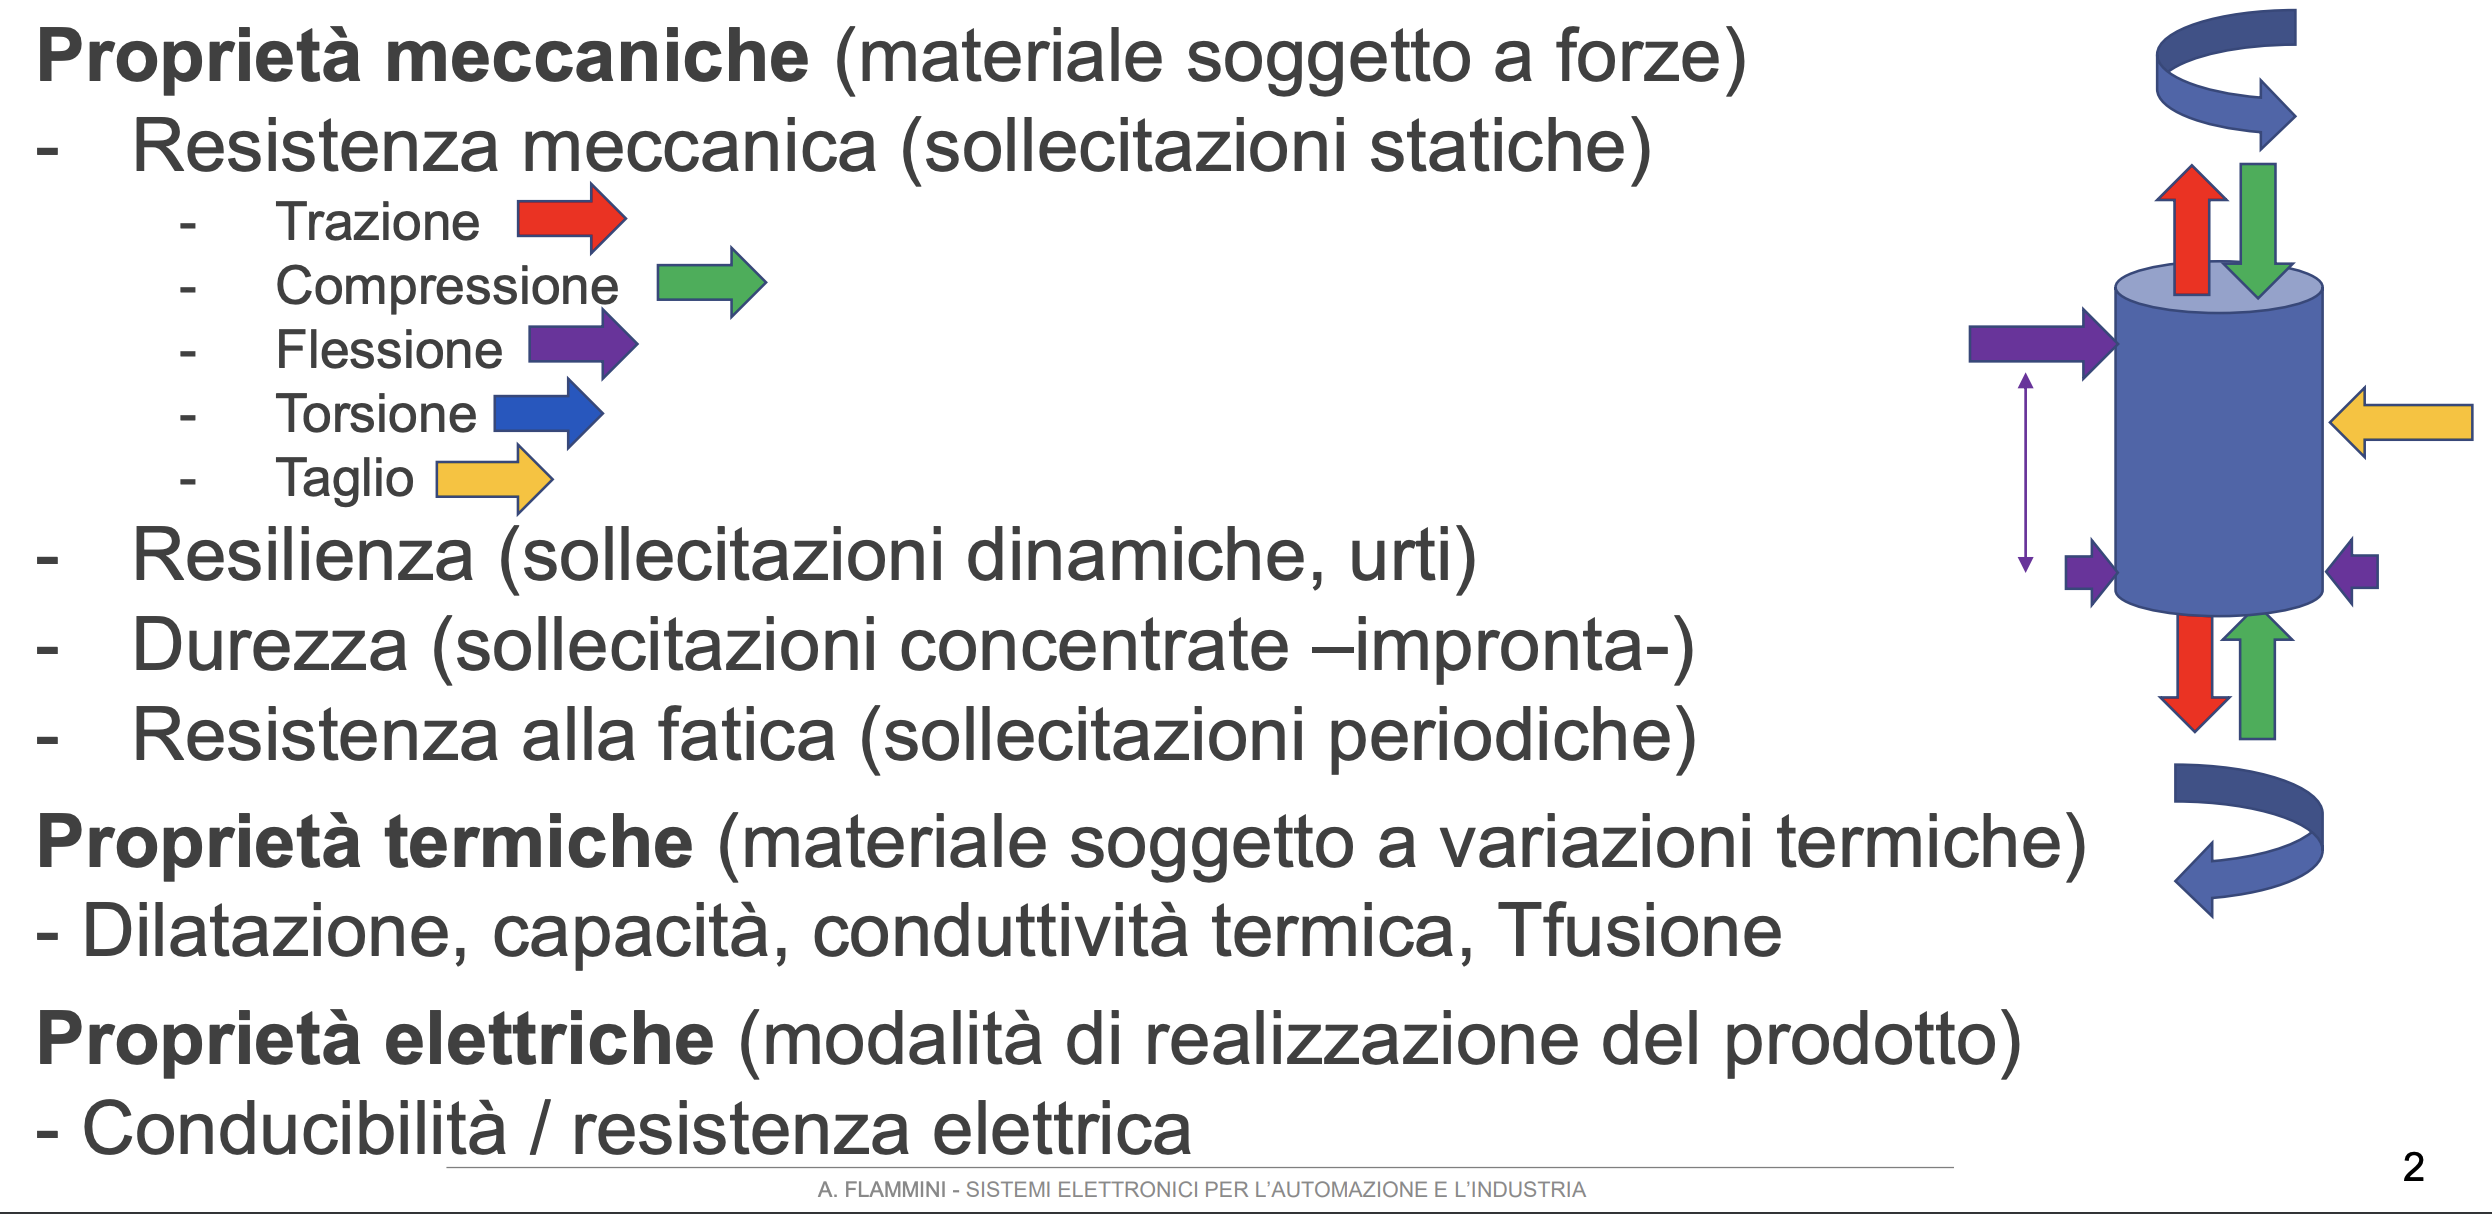
\includegraphics[width=0.5\textwidth]{mecc1.png}
\end{figure}
\subsection{Materiali tipici}
\begin{itemize}
    \item Metalli: acciaio, alluminio, rame
    \item Legno: non inquinante, riassorbito dall'ambiente
    \item Plastica: fortemente inquinante, microplastiche che persistono nell'ambiente. Riciclo plastica trasformandola in un impasto e ridandole una forma oppure in un filamento e utilizzato per le stampe 3d
    \item Materiali organici: food\&beverage
    \item Materiali chimici: pharma\&beauty (simile alla farmaceutica)
\end{itemize}
\subsection{Processi metallurgici}
\begin{itemize}
    \item Materie prime: \begin{itemize}
        \item carbone
        \item minerale
    \end{itemize}
\end{itemize}
\begin{figure}
    \centering
    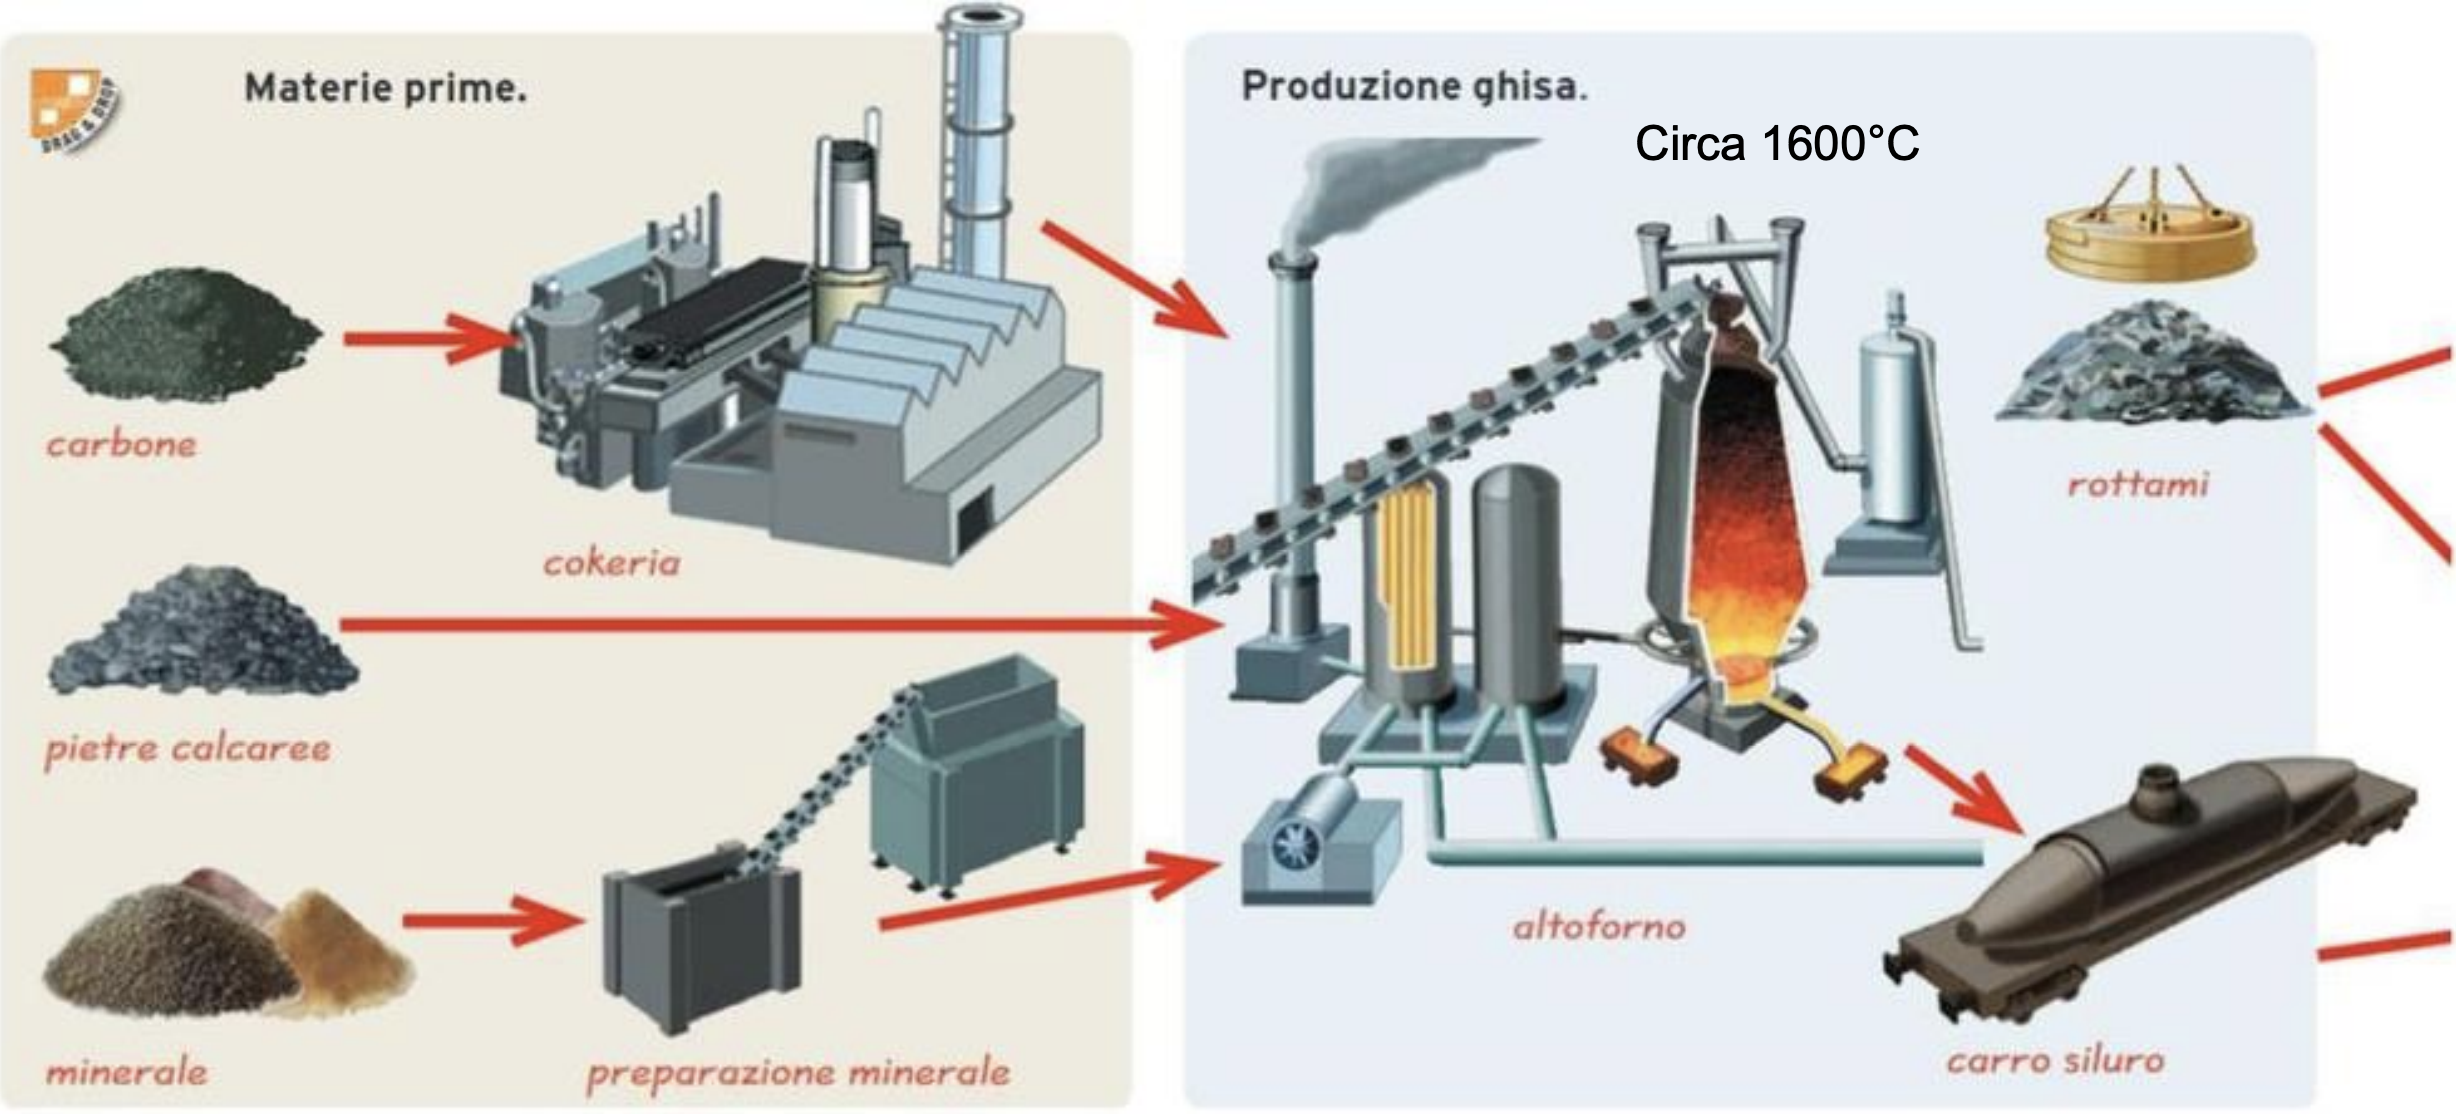
\includegraphics[width=0.5\textwidth]{mecc2.png}
    Grande potenza poca automazione $\implies$ non è una fabbrica, ma un impianto di processo.
\end{figure}
\begin{figure}
    \centering
    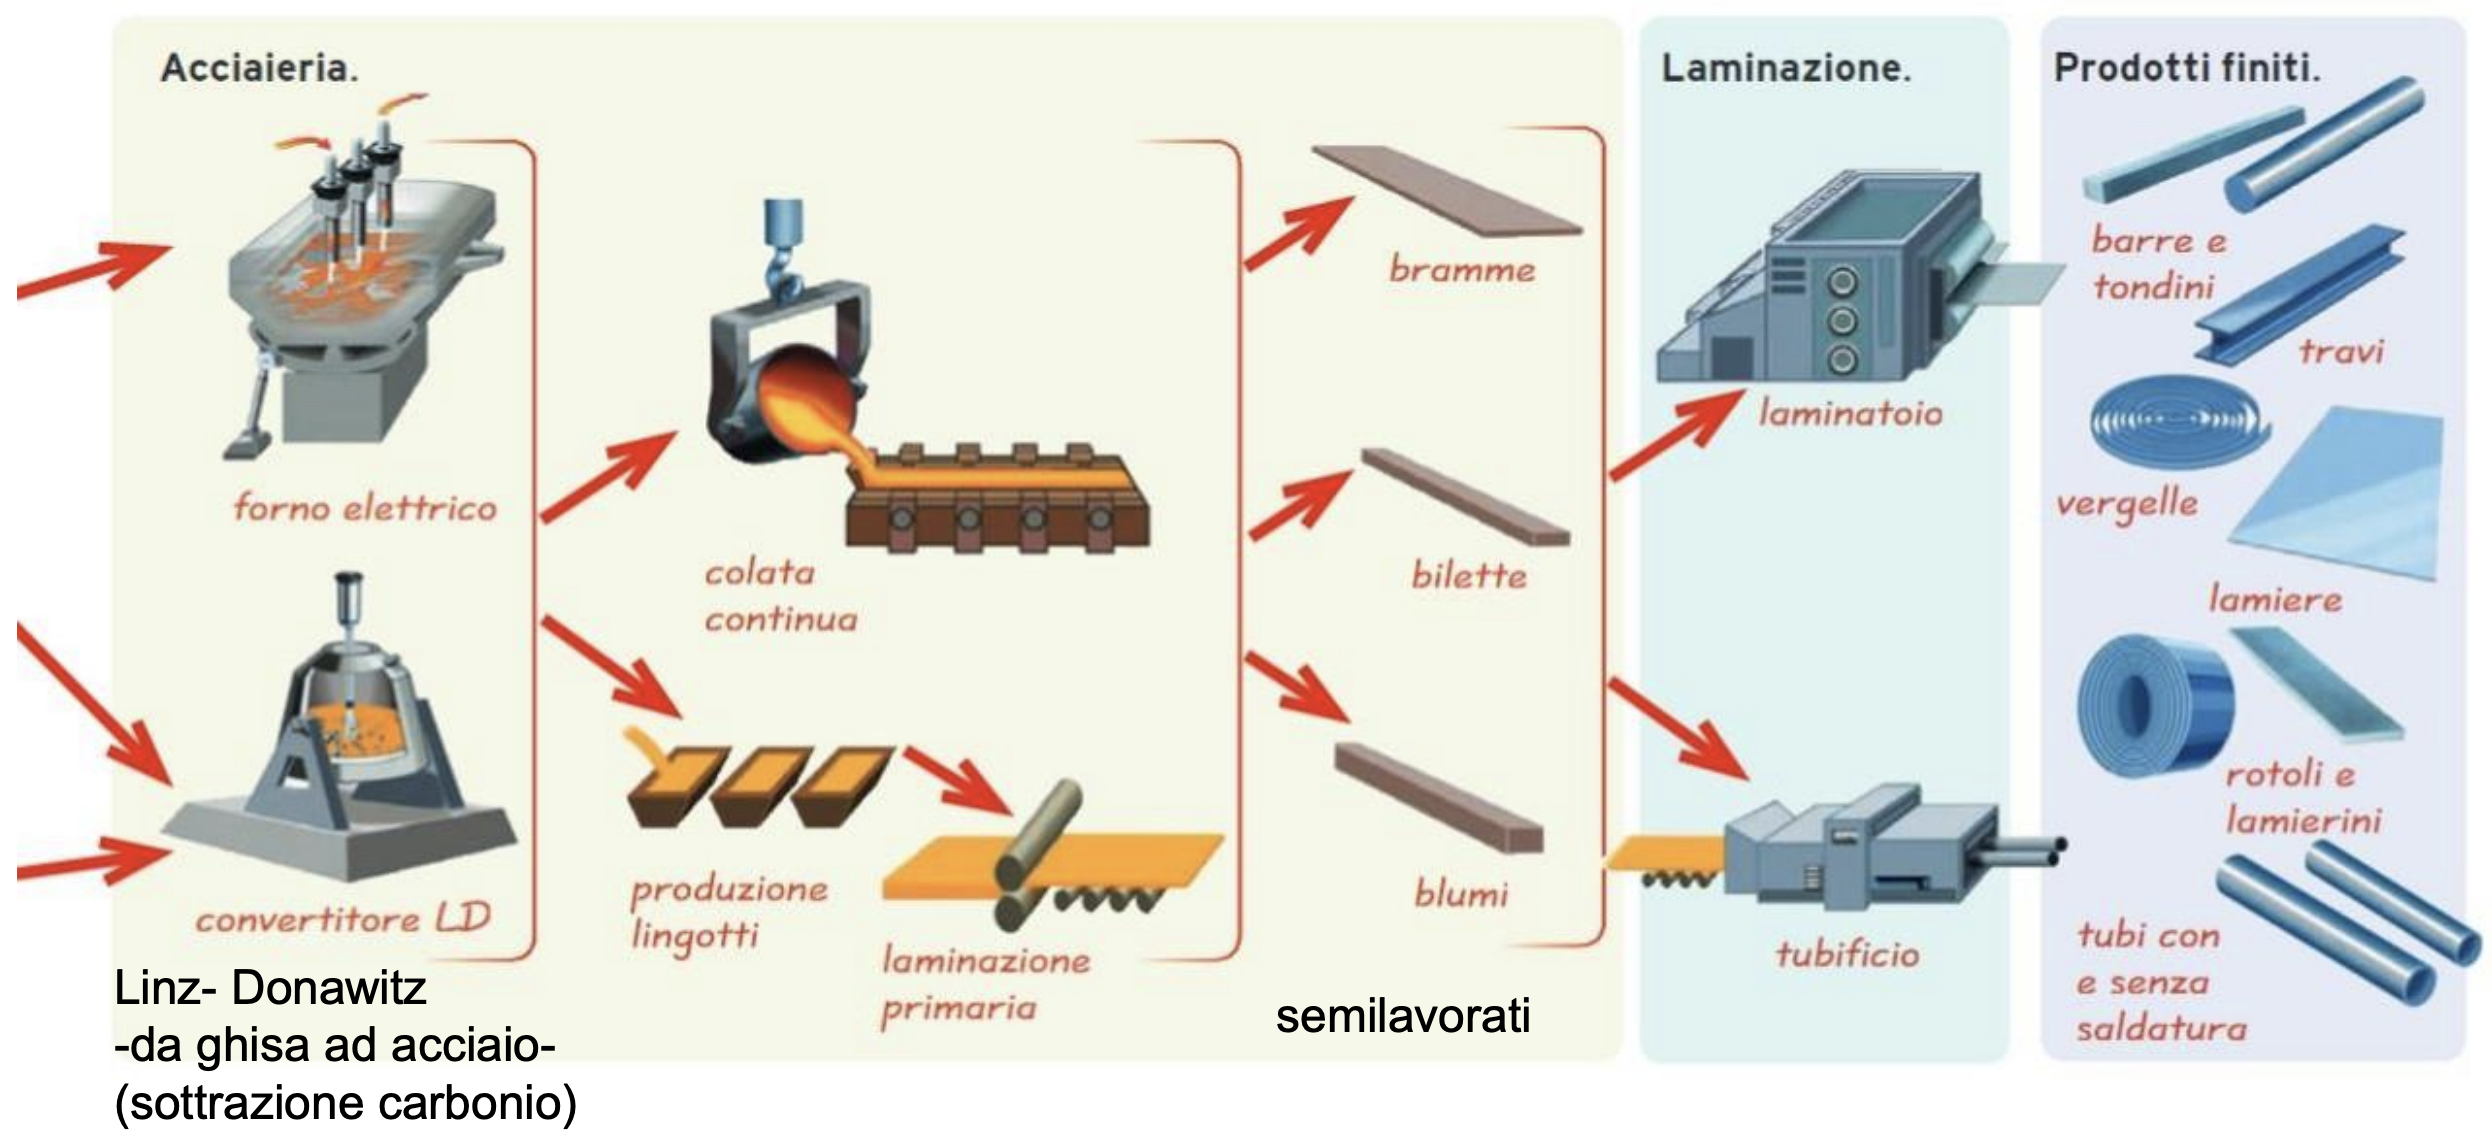
\includegraphics[width=0.5\textwidth]{mecc3.png}
    Tramite lavorazioni primarie ottengo dei semilavorati.
\end{figure}
\begin{itemize}
    \item Bramme $\implies$ lamiere tramite laminazioni per assottigliarle
    \item Bilette $\implies$ barre e tondini (o vergella, molto più sottile)
    \item Blumi $\implies$ tubi mediante foratura (il tubo si può ottenere anche tramite saldatura di una lamiera)
\end{itemize}
\subsection{Lavorazioni e trattamenti}
Il materiale prodotto da lavorazioni per esportazione si chiama \textbf{truciolo}, che è un sottoprodotto in quanto poi viene fuso e riutilizzato.

meccanica toglie materiale
plastica lo modella










\end{document}